\documentclass[11pt,fleqn]{article} 
\usepackage[margin=0.8in, head=0.8in]{geometry} 
\usepackage{amsmath, amssymb, amsthm}
\usepackage{fancyhdr} 
\usepackage{palatino, url, multicol}
\usepackage{graphicx} 
\usepackage[all]{xy}
\usepackage{polynom} 
\usepackage{pdfsync}
\usepackage{enumerate}
\usepackage{framed}
\usepackage{setspace}
\usepackage{array,tikz,pgfplots}
%%yikz plots
\usetikzlibrary{calc}
\pgfplotsset{my style/.append style={axis x line=middle, axis y line=
middle, xlabel={$x$}, ylabel={$y$}, axis equal }}

\pagestyle{fancy} 
\lfoot{UAF Calculus 1}
\rfoot{1-5 Trigonometry}

\begin{document}
\setlength{\parindent}{0cm}
\renewcommand{\headrulewidth}{0pt}
\newcommand{\blank}[1]{\rule{#1}{0.75pt}}
\renewcommand{\d}{\displaystyle}
\vspace*{-0.9in}
\begin{center}
  \LARGE \sc{Lecture: 1-3: Transformations and Trigonometry Review}
\end{center}
\small
\begin{enumerate}

\subsection*{Transformation Review}
\item Explain what each does to the \emph{original} graph $y=f(x).$ (Assume $c > 0.$)
\begin{multicols}{2}
\begin{enumerate}
\item $f(x)+c$\\

\item $f(x)-c$\\
\item $f(x+c)$\\
\item $f(x-c)$\\
\item $cf(x)$\\
\item $f(cx)$\\
\item $-f(x)$\\
\item $f(-x)$\\
\end{enumerate}
\end{multicols}
\item Let $f(x)=\begin{cases} 2 & x \leq 1 \\ 3-x & x > 1 \end{cases}.$ Graph each of the following \emph{using the ideas from \# 1 above.}
\begin{multicols}{2}

\begin{enumerate}
\item $f(x)$\\
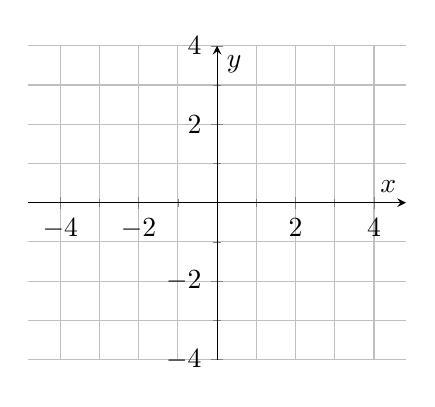
\begin{tikzpicture}
\begin{axis}[scale=0.7, my style, xtick={-4,-2,...,4}, ytick={-4,-2,...,4},
xmin=-4, xmax=4, ymin=-4, ymax=4, grid=both, minor y tick num=1,
        minor x tick num=1, mark size=3.0pt]
%\addplot[domain=0:2,ultra thick] {x};
%\addplot[domain=2:4, ultra thick] {-2*x+6};
%\addplot[domain=4:5, ultra thick] {-2};
\end{axis}
\end{tikzpicture}

\item $f(x+1)$\\
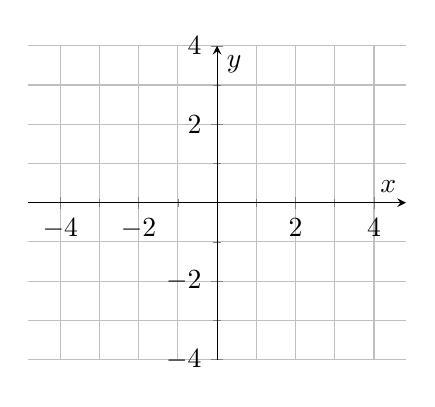
\begin{tikzpicture}
\begin{axis}[scale=0.7, my style, xtick={-4,-2,...,4}, ytick={-4,-2,...,4},
xmin=-4, xmax=4, ymin=-4, ymax=4, grid=both, minor y tick num=1,
        minor x tick num=1, mark size=3.0pt]
%\addplot[domain=0:2,ultra thick] {x};
%\addplot[domain=2:4, ultra thick] {-2*x+6};
%\addplot[domain=4:5, ultra thick] {-2};
\end{axis}
\end{tikzpicture}

\item $f(2x)$\\
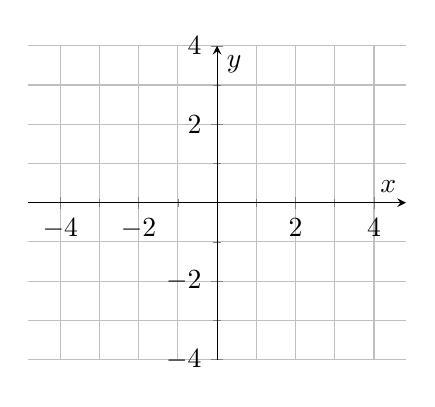
\begin{tikzpicture}
\begin{axis}[scale=0.7, my style, xtick={-4,-2,...,4}, ytick={-4,-2,...,4},
xmin=-4, xmax=4, ymin=-4, ymax=4, grid=both, minor y tick num=1,
        minor x tick num=1, mark size=3.0pt]
%\addplot[domain=0:2,ultra thick] {x};
%\addplot[domain=2:4, ultra thick] {-2*x+6};
%\addplot[domain=4:5, ultra thick] {-2};
\end{axis}
\end{tikzpicture}

\item $-2f(x)$\\
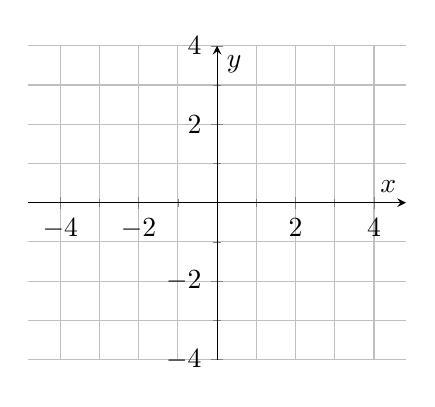
\begin{tikzpicture}
\begin{axis}[scale=0.7, my style, xtick={-4,-2,...,4}, ytick={-4,-2,...,4},
xmin=-4, xmax=4, ymin=-4, ymax=4, grid=both, minor y tick num=1,
        minor x tick num=1, mark size=3.0pt]
%\addplot[domain=0:2,ultra thick] {x};
%\addplot[domain=2:4, ultra thick] {-2*x+6};
%\addplot[domain=4:5, ultra thick] {-2};
\end{axis}
\end{tikzpicture}

\end{enumerate}
\end{multicols}
\newpage


\subsection*{Three Views of Trigonometric Functions} 
\begin{itemize}
\item sides of a right triangle
\item points on the unit circle
\item graphs in the $xy$-plane
\end{itemize}

\subsubsection*{The Triangle Defintion}

\item Sketch a right triangle with side $a$ adjacent to an
angle $\theta$, $o$ opposite of the angle $\theta$ and hypotenuse
$h$. Define each of the six trigonometric functions in terms of that
triangle. 


  \begin{multicols}{6}{
      % make sure you added \usepackage{enumerate}
      \vspace*{-0.45in}
      \begin{enumerate}[a)]
      \item $\sin \theta$
      \item $\cos \theta$
      \item $\tan \theta$
      \item $\sec \theta$
      \item $\csc \theta$
      \item $\cot \theta$
      \end{enumerate}}
  \end{multicols}

\vskip1in

\item An isosceles triangle has a height of 10 ft and its base is 8 feet long. Determine the sine, cosine and tangent of the base angle.
\vfill

\subsubsection*{The Unit Circle Approach}

\item Using a 45-45-90 triangle and a 30-60-90 triangle
find the coordinates of ALL of the points on the unit circle.
\begin{flushleft}
  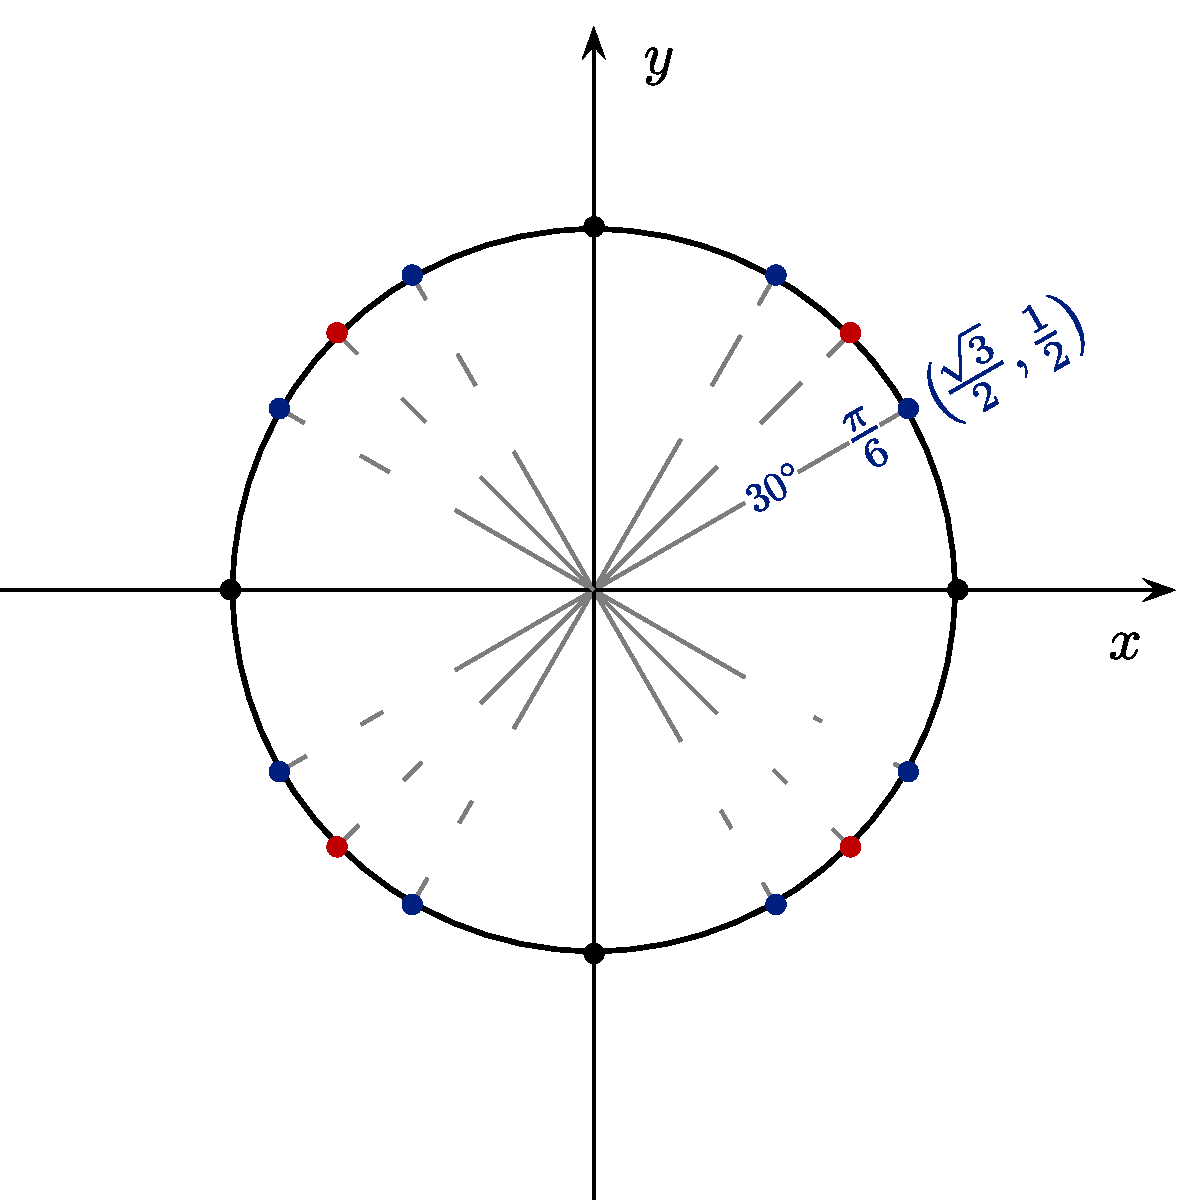
\includegraphics[width=3.5in]{blank-unit-circle}
\end{flushleft}

\newpage
\vspace*{-0.9in}
\item Without a calculator evaluate:
  \begin{multicols}{3}{
      % make sure you added \usepackage{enumerate}
      \vspace*{-0.45in}
      \begin{enumerate}[(a)]
      \item $\sin (\frac{2 \pi}{3} )$
      \item $\cos( \frac{5 \pi}{4} )$
      \item $\tan(\frac{- \pi}4 )$
      \end{enumerate}}
  \end{multicols}

\vskip1in

\item On the axes below, graph \emph{at least two cycles} of $f(x)=\sin x,$ $f(x)=\cos x,$ and $f(x)=\tan x.$ Label all $x$- and $y$-intercepts.\\
\vfill
 \begin{tabular}{lcr}
 \begin{tikzpicture}[scale=.8]
 \draw[<->] (-4,0) -- (4,0);
 \draw[<->]  (0,-2) -- (0,2);
 \end{tikzpicture}
 &\quad \hspace{.4in} \quad &
 \begin{tikzpicture}[scale=.8]
 \draw[<->] (-4,0) -- (4,0);
 \draw[<->]  (0,-2) -- (0,2);
 \end{tikzpicture}
  \end{tabular}

\vfill
 \begin{tikzpicture}[scale=.7]
 \draw[<->] (-2,0) -- (5,0);
 \draw[<->]  (0,-3) -- (0,3);
 \end{tikzpicture}
\vfill

\item Use the graphs above to solve the equations below.
\begin{multicols}{2}
\begin{enumerate}
\item $\cos x =1$
\vspace{.5in}
\item $\sin x =1$
\vspace{1in}
\columnbreak
\item $\tan x = 0$
\vspace{1in}
\item $\sin x = 1/2$ (Find all solutions in $[0,2\pi].$)
\vspace{.5in}
\end{enumerate}
\end{multicols}
\vspace{.5in}
\newpage
\item For each problem below, sketch the graph and use it to help you solve the equation or answer the question.
\begin{enumerate}
\item Graph $y=\sin(x-1)$ and use it to solve the equation $\sin(x-1)=1.$
\vfill
\item Graph $y=\sin(x/2)$ and use it to find the domain of  $f(x)=\csc(x/2).$
\vfill
\item Graph $y=-2\cos(x)$ and use it to solve the equation $-2\cos(x)=0.$
\vfill
\end{enumerate}

\end{enumerate}
\end{document}
\textbf{Example 5:} Find the following values. 

  \begin{multicols}{3}{
      % make sure you added \usepackage{enumerate}
      \vspace*{-0.45in}
      \begin{enumerate}[(a)]
      \item $\tan( \frac{3 \pi}4)$
      \item $\cot( \frac{\pi}{6})$
      \item $\sec(\pi)$
      \end{enumerate}}
  \end{multicols}

\vskip1in

\textbf{Example 6:} Graph the following functions on $[- \pi, \pi ]$. Clearly label any asymptotes.

  \begin{multicols}{2}{
      % make sure you added \usepackage{enumerate}
      \vspace*{-0.45in}
      \begin{enumerate}[a)]
      \item $f(x) = \tan x$

\begin{tikzpicture}[scale=0.65][>=latex]
%x axis
\draw[->] (-5 ,0) -- (5 ,0) node[below] {$x$};
\foreach \x in {-4,...,4}
\draw[shift={(\x,0)}] (0pt,2pt) -- (0pt,-2pt);
%y axis
\draw[->] (0,-2.5) -- (0,2.5) node[left] {$y$};
\foreach \y in {-1,...,1}
\draw[shift={(0,\y)}] (2pt,0pt) -- (-2pt,0pt);
% \node[below left] at (0,0) {\footnotesize $0$};
\end{tikzpicture}


      \item $f(x) = \cot x$

\begin{tikzpicture}[scale=0.65][>=latex]
%x axis
\draw[->] (-5 ,0) -- (5 ,0) node[below] {$x$};
\foreach \x in {-4,...,4}
\draw[shift={(\x,0)}] (0pt,2pt) -- (0pt,-2pt);
%y axis
\draw[->] (0,-2.5) -- (0,2.5) node[left] {$y$};
\foreach \y in {-1,...,1}
\draw[shift={(0,\y)}] (2pt,0pt) -- (-2pt,0pt);
% \node[below left] at (0,0) {\footnotesize $0$};
\end{tikzpicture}

      \end{enumerate}}
  \end{multicols}

\vfill

\textbf{Example 7:} Graph the following functions on $[- 2 \pi, 2
\pi]$. Clearly label any asymptotes. 


  \begin{multicols}{2}{
      % make sure you added \usepackage{enumerate}
      \vspace*{-0.45in}
      \begin{enumerate}[a)]
      \item $f(x) = \sec x$

\begin{tikzpicture}[scale=0.65][>=latex]
%x axis
\draw[->] (-5 ,0) -- (5 ,0) node[below] {$x$};
\foreach \x in {-4,...,4}
\draw[shift={(\x,0)}] (0pt,2pt) -- (0pt,-2pt);
%y axis
\draw[->] (0,-2.5) -- (0,2.5) node[left] {$y$};
\foreach \y in {-1,...,1}
\draw[shift={(0,\y)}] (2pt,0pt) -- (-2pt,0pt);
% \node[below left] at (0,0) {\footnotesize $0$};
\end{tikzpicture}


      \item $f(x) = \csc x$

\begin{tikzpicture}[scale=0.65][>=latex]
%x axis
\draw[->] (-5 ,0) -- (5 ,0) node[below] {$x$};
\foreach \x in {-4,...,4}
\draw[shift={(\x,0)}] (0pt,2pt) -- (0pt,-2pt);
%y axis
\draw[->] (0,-2.5) -- (0,2.5) node[left] {$y$};
\foreach \y in {-1,...,1}
\draw[shift={(0,\y)}] (2pt,0pt) -- (-2pt,0pt);
% \node[below left] at (0,0) {\footnotesize $0$};
\end{tikzpicture}
      \end{enumerate}}
  \end{multicols}

\vfill


\newpage


\subsubsection*{Common Identities} 

When you first learned trigonometry you probably had to prove a bunch
of equivalencies using various identities. Perhaps you discussed why
these identies were true. Some of you may have been asked to memorize
all of these and some of you may have been allowed a note card/ cheat
sheet. In this class you need to have the following \textbf{SIX}
identities and no more. 

\textbf{The Pythagorean Identities:} Looking at the unit circle,
derive an identity involving sine and cosine using the pythagorean
theorem. This is (a). Next, divide the answer to (a) by $\cos^2
\theta$ to obtain a new identity for (b). Finally, divide (a) by
$\sin^2 \theta$ to obtain the third Pythagorean identity for (c). 


  \begin{multicols}{3}{
      % make sure you added \usepackage{enumerate}
      \vspace*{-0.45in}
      \begin{enumerate}[(a)]
      \item Identity $\# 1$
      \item Identity $\# 2$
      \item Identity $\# 3$
      \end{enumerate}}
  \end{multicols}
\vskip1.2in

\textbf{The Half/ Double Angle Identities:} You have probably seen the
identities $\cos(2 \theta) = 1 - 2 \sin^2 \theta$ and $\cos(2 \theta)
= 1 + 2 \cos^2 \theta$. It is more likely that we will use these
slightly differently in this class. Solve these identities for $\sin^2
\theta$ and $\cos^2 \theta$ respectively. Finally, given an identity
for $\sin(2 \theta)$. 


  \begin{multicols}{3}{
      % make sure you added \usepackage{enumerate}
      \vspace*{-0.45in}
      \begin{enumerate}[(a)]
      \item $\cos(2 \theta) = 1 - 2 \sin^2 \theta$
      \item $\cos(2 \theta) = 1 + 2 \cos^2 \theta$
      \item $\sin(2 \theta)$
      \end{enumerate}}
  \end{multicols}
\vskip1.2in



  \subsection*{Inverse Trigonometric Functions}




  \textbf{Definition and graphs of $\sin^{-1} x$ and $\cos^{-1} x$}


\vskip1.5in


  \textbf{Example 9:} Evaluate the following expressions.


  \begin{multicols}{3}{
      % make sure you added \usepackage{enumerate}
      \vspace*{-0.35in}
      \begin{enumerate}[(a)]
      \item $\sin^{-1}(\sqrt 3/ 2)$
      \item $\cos^{-1} (-1/2)$
      \item $\tan(\arcsin 1/5)$
      \end{enumerate}}
  \end{multicols}

 
  \vskip1.5in







  \textbf{Definition and graph of $\tan^{-1} x$}


\vskip1.5in




  \textbf{Example 10:} Simplify the following expressions.


  \begin{multicols}{3}{
      % make sure you added \usepackage{enumerate}
      \vspace*{-0.35in}
      \begin{enumerate}[a)]
      \item $\tan^{-1} (-1)$
      \item $\tan^{-1} (\sqrt 3)$
      \item $\tan^{-1} 0$
      \end{enumerate}}
  \end{multicols}


\vskip0.5in
\textbf{Example 11:} Simplify the following expressions. 

  \begin{multicols}{2}{
      % make sure you added \usepackage{enumerate}
      \vspace*{-0.45in}
      \begin{enumerate}[a)]
      \item $\sin(\tan^{-1} \frac x 2 )$
      \item $\sin(2 \arccos x)$
      \end{enumerate}}
  \end{multicols}

\vskip1.5in

\textbf{Example 12:} How is $\tan^{-1} (1)$ different from solving the
equation $\tan x = 1$? Why does the former have only one value while
the latter has an infinite number of values?
\vskip1.5in

\textbf{Example 13:} Are the following statements true or false? 


  \begin{multicols}{3}{
      % make sure you added \usepackage{enumerate}
      \vspace*{-0.45in}
      \begin{enumerate}[(a)]
      \item $\sin^{-1} x = \frac{1}{\sin x}$
      \item $\tan^{-1} (-1) = \frac{3 \pi}{4}, \frac{7 \pi}{4}$
      \item $\sin^2 x = 1 + \cos^2 x$
      \end{enumerate}}
  \end{multicols}



\end{enumerate}



\end{document}